\chapter{Descrizione generale del progetto}

\begin{preamble}
{\em 
Nel terzo capitolo si presenterà una panoramica del progetto di questa tesi. Si inizierà con una breve introduzione relativa al suo scopo generale. Successivamente, si approfondiranno i dettagli relativi agli strumenti software utilizzati nel progetto, tra cui Unity, Vuforia Engine, Polycam, Blender, Vuforia Model Target Generator, MongoDB, Google Earth Studio e OpenWeather. \newline \indent In seguito, si esplorerà nel dettaglio la stazione IoT situata nel vigneto della cantina Strappelli, che è stata messa a disposizione per il monitoraggio dei dati relativi al vigneto. In aggiunta, si fornirà una breve illustrazione del funzionamento dell'applicazione, descrivendo tutte le fasi che vanno dal lancio del menu principale fino alla visualizzazione dei dati relativi al vigneto associato al prodotto vitivinicolo riconosciuto dall'applicazione. Il tutto verrà illustrato fornendo degli screenshot per facilitare la comprensione di quello che verrà descritto.
}
\end{preamble}

\section{Premessa}

In questo capitolo, si esplorerà in dettaglio la creazione di un'app mobile per dispositivi Android. Questa app avrà la capacità di riconoscere automaticamente prodotti vitivinicoli attraverso la fotocamera dello smartphone, mettendo particolare enfasi sulle bottiglie di vino. Un elemento chiave è che il riconoscimento non si baserà sui tradizionali codici QR, ma farà uso di modelli tridimensionali degli oggetti precedentemente caricati all'interno dell'applicazione in modo tale da non alterare le etichette delle bottiglie per far funzionare l'applicazione. Una volta completata con successo la fase di riconoscimento, l'app fornirà all'utente informazioni dettagliate sul prodotto identificato.

\section{Scopo generale dell'applicazione}

Lo scopo dell'applicazione è quello di fornire informazioni sul vigneto di provenienza delle bottiglie di vino riconosciute, combinando i dati dell'azienda Trace Technologies con dati satellitari provenienti dall'API di OpenWeather. La struttura dei dati utilizzati sarà descritta nel quarto capitolo.

Una volta effettuato il riconoscimento, l'app sarà suddivisa in tre sezioni principali:

\begin{itemize}
    \item \textit{Osserva}: in questa sezione, gli utenti avranno a disposizione una ricca fonte di informazioni, sia testuali che multimediali, relative al prodotto vitivinicolo appena identificato. Sarà possibile esplorare il nome della cantina produttrice, avere una breve descrizione del vino, nonché dettagli informativi sul luogo in cui esso è stato prodotto. Inoltre, per offrire un'esperienza visiva coinvolgente, l'app presenterà un breve video che fornirà una vista panoramica dall'alto, sfruttando immagini satellitari ottenute da Google Earth Studio, del luogo di produzione del prodotto vitivinicolo.
    \item \textit{Ascolta}: questa sezione opera in modo simile a un karaoke, ma con una differenza fondamentale: gli utenti potranno godere di una recensione testuale del vino, redatta da un sommelier esperto, sincronizzata in tempo reale con l'audio fornito dallo stesso sommelier. Questa caratteristica rappresenta un notevole miglioramento dell'esperienza dell'utente, arricchendo l'interazione con l'app in modo significativo.
    \item \textit{Racconta}: l'ultima sezione è dedicata alla visualizzazione dello stato di salute del vigneto di provenienza delle bottiglie di vino. Questa sezione si divide in due parti essenziali; la prima parte fornisce dati provenienti dalla stazione IoT di Trace Technologies, inclusi parametri come temperatura e umidità ambientale, quantità giornaliera di pioggia, temperatura delle foglie e umidità delle foglie del vigneto. La seconda parte presenta lo stato di salute del vigneto utilizzando dati ottenuti dall'API OpenWeather.

\end{itemize}

\section{Strumenti software utilizzati}

\subsection{Unity}

\textit{Unity} (Figura \ref{3fig:logo_unity}) è una delle piattaforme di sviluppo di giochi e simulazioni più potenti e versatili disponibili oggi. È un ambiente di sviluppo integrato (IDE) che offre agli sviluppatori una vasta gamma di strumenti e risorse per creare giochi, applicazioni interattive e simulazioni per una vasta gamma di piattaforme, compresi PC, console, dispositivi mobili, realtà virtuale (VR) e realtà aumentata (AR).

\begin{figure}[h]
	\centering
	
\includegraphics [width=.40\columnwidth, angle=0]
            {logoUnity}
	\caption{Logo di Unity}
	\label{3fig:logo_unity}
\end{figure}

\subsubsection{Storia di Unity}

La storia di Unity risale al 2005, quando fu sviluppato da David Helgason, Joachim Ante e Nicholas Francis. Da allora, Unity Technologies ha continuato a crescere ed evolversi, diventando uno dei leader nel settore dello sviluppo di giochi e applicazioni 3D. Attualmente, Unity è utilizzato da milioni di sviluppatori in tutto il mondo, dai principianti agli sviluppatori esperti.

\subsubsection{Aspetti distintivi e funzionalità}

Uno degli aspetti distintivi di Unity è la sua flessibilità. Esso supporta una vasta gamma di linguaggi di programmazione, tra cui C\ e JavaScript, consentendo agli sviluppatori di utilizzare il linguaggio con cui si sentono più a loro agio. Questa flessibilità rende Unity un'ottima scelta per sviluppatori con diverse competenze ed esperienze.

Unity offre una serie di funzionalità e strumenti avanzati, tra cui:

\begin{itemize}
    \item \textit{Grafica avanzata}: Unity supporta una grafica di alta qualità con rendering in tempo reale, illuminazione globale, riflessi, ombre dinamiche e supporto per il ray tracing. Gli sviluppatori possono creare mondi virtuali incredibilmente dettagliati e realistici.
    \item \textit{Fisica realistica}: Unity include un motore fisico avanzato che consente agli sviluppatori di simulare il comportamento realistico degli oggetti, dalla caduta degli oggetti alla dinamica dei veicoli.
    \item \textit{Animazione}: gli sviluppatori possono creare animazioni complesse per personaggi e oggetti utilizzando il sistema di animazione di Unity, che supporta la blend tree, l'animazione retargeting e altro ancora.
    \item \textit{Intelligenza artificiale}: Unity offre strumenti per la creazione di comportamenti di Intelligenza Artificiale (IA) per personaggi non giocanti e avversari controllati dall'IA.
    \item \textit{Realtà virtuale e aumentata}: Unity è una scelta popolare per lo sviluppo di applicazioni VR e AR, con supporto integrato per numerosi dispositivi e librerie di sviluppo.
    \item \textit{Multi-piattaforma}: gli sviluppatori possono creare giochi e applicazioni per una vasta gamma di piattaforme, compresi \textit{Windows}, \textit{macOS}, \textit{Linux}, \textit{iOS}, \textit{Android}, \textit{PlayStation}, \textit{Xbox} e molte altre.
    \item \textit{Asset Store}: Unity dispone di un Asset Store che offre una vasta selezione di risorse pronte all'uso, come modelli 3D, suoni, effetti speciali e plugin, che possono accelerare notevolmente il processo di sviluppo. 
    \item \textit{Community e supporto}: Unity ha una vasta comunità di sviluppatori attivi, forum di supporto e una documentazione dettagliata che aiutano gli sviluppatori a risolvere i problemi e a imparare nuove tecniche.
\end{itemize}

Inoltre, Unity è utilizzato in una varietà di settori oltre ai videogiochi, tra cui l'architettura, la simulazione, la formazione, la medicina e l'arte interattiva. La sua versatilità e la sua capacità di adattarsi a una vasta gamma di progetti lo rendono uno strumento eccezionale per chiunque desideri creare esperienze digitali coinvolgenti e interattive.

\subsection{Vuforia Engine}

\textit{Vuforia Engine} (Figura \ref{3fig:logo_vuforia}) è una potente piattaforma di realtà aumentata (AR) sviluppata da \textit{PTC (Parametric Technology Corporation)} che consente agli sviluppatori di creare applicazioni AR immersive e interattive per una vasta gamma di dispositivi e piattaforme. Questo strumento è stato utilizzato in molte applicazioni, tra cui giochi, applicazioni industriali, educative e di marketing, per portare il mondo fisico e il digitale insieme in modo innovativo.

\begin{figure}[h]
	\centering
	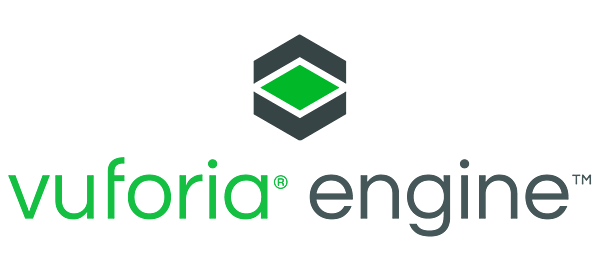
\includegraphics [width=.45\columnwidth, angle=0]
            {logoVuforia}
	\caption{Logo di Vuforia Engine}
	\label{3fig:logo_vuforia}
\end{figure}

\subsubsection{Caratteristiche di Vuforia Engine}

Le caratteristiche principali di Vuforia Engine sono:

\begin{itemize}
    \item \textit{Rilevamento degli oggetti e dei marker}: una delle caratteristiche chiave di Vuforia Engine è la sua capacità di rilevare oggetti fisici o marker grafici nel mondo reale e di tracciare la loro posizione e orientamento. Questo avviene attraverso la visione computerizzata e l'analisi dell'immagine catturata dalla fotocamera del dispositivo AR. I marker possono essere stampati su carta o inseriti in oggetti reali. 
    \item \textit{Tracciamento dei movimenti}: Vuforia Engine offre anche funzionalità di tracciamento dei movimenti, consentendo agli oggetti AR di rimanere ancorati al loro punto di riferimento anche quando l'utente si sposta. Questo è fondamentale per garantire un'esperienza AR fluida e realistica. 
    \item \textit{Riconoscimento dell'ambiente}: oltre al rilevamento di marker, Vuforia Engine può riconoscere l'ambiente circostante, consentendo agli oggetti AR di interagire con gli elementi reali dell'ambiente. Ad esempio, un'applicazione AR può posizionare un oggetto virtuale su un tavolo o farlo interagire con una parete.
    \item \textit{Rendering 3D}: una volta che Vuforia Engine ha acquisito e tracciato le informazioni sull'ambiente e sugli oggetti, può visualizzare oggetti 3D virtuali nell'ambiente del mondo reale. Questo processo di rendering 3D viene effettuato in tempo reale per garantire che gli oggetti AR si integrino perfettamente nell'ambiente. 
    \item \textit{Interazione utente}: Vuforia Engine offre anche supporto per l'interazione utente. Gli utenti possono interagire con gli oggetti AR attraverso gesti, tocchi e input vocali, consentendo loro di manipolare oggetti virtuali e di ricevere risposte dall'applicazione. 
    \item \textit{Multi-piattaforma}: Vuforia Engine è compatibile con una vasta gamma di dispositivi, tra cui smartphone, tablet, occhiali AR e HoloLens di Microsoft. Questa flessibilità consente agli sviluppatori di creare applicazioni AR che raggiungono un pubblico ampio e diversificato. 
    \item \textit{Sicurezza e privacy}: Vuforia Engine si preoccupa della sicurezza e della privacy degli utenti, garantendo che le applicazioni AR rispettino le normative sulla protezione dei dati e consentano agli utenti di controllare le autorizzazioni per l'accesso alla fotocamera e ad altre informazioni personali. 
    \item \textit{Supporto per lo sviluppatore}: Vuforia Engine offre una serie di strumenti e risorse per gli sviluppatori, tra cui un'ampia documentazione, esempi di codice, un'interfaccia di sviluppo intuitiva e un'attiva community online. Ciò facilita la creazione di applicazioni AR di alta qualità.
\end{itemize}

\subsection{Polycam}

\textit{Polycam} (Figura \ref{3fig:logo_polycam}) è un'applicazione mobile in grado di generare un modello tridimensionale a partire da una sequenza di foto scattate con il proprio smartphone.

\begin{figure}[h]
	\centering
	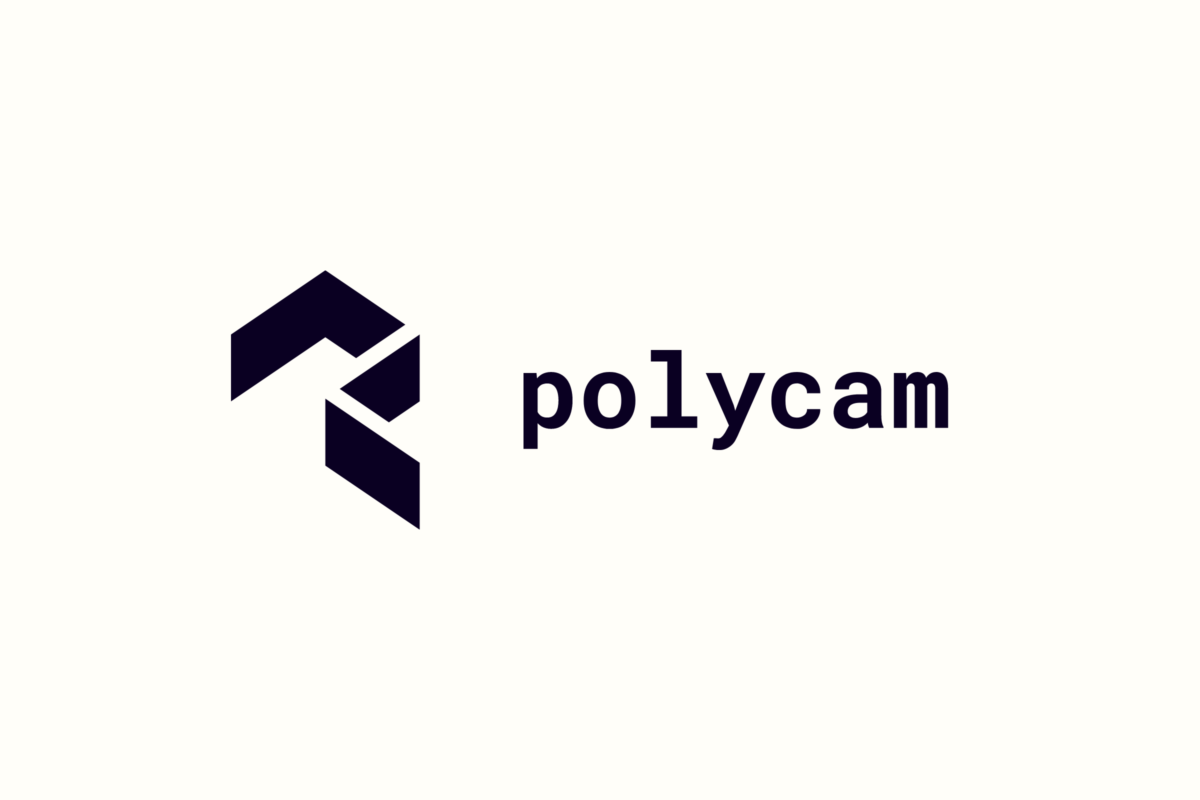
\includegraphics [width=.35\columnwidth, angle=0]
            {logoPolycam}
	\caption{Logo di Polycam}
	\label{3fig:logo_polycam}
\end{figure}

Esistono quattro modi diversi per creare una scansione in Polycam. Questi sono descritti di seguito:

\begin{itemize}
    \item \textit{Photo Mode}: è di solito la scelta migliore per gli oggetti che richiedono una grande precisione e un grande dettaglio, o quando non si ha accesso a un sensore LiDAR. Questo metodo funziona scattando una sequenza di fotografie standard dell'oggetto che vengono poi caricate in un server più potente che crea la ricostruzione tridimensionale con la massima precisione possibile.
    \item \textit{LiDAR Mode}: è una modalità comoda per l'acquisizione di spazi o quando si desidera effettuare una scansione rapidamente. Il metodo utilizza i dati di profondità forniti dal sensore LiDAR che permette di generare una ricostruzione tridimensionale dell'ambiente direttamente sul dispositivo. Questo approccio sfrutta le capacità di misurazione precisa del sensore LiDAR per ottenere risultati veloci e affidabili nella creazione di modelli 3D.
    \item \textit{Room Mode}: questa modalità consente di generare planimetrie professionali in 3D e 2D e di misurare istantaneamente gli spazi interni.
    \item \textit{360 Mode}: questa modalità permette di scattare foto panoramiche a 360$^{\circ}$ con l'ausilio dell'Intelligenza Artificiale.
\end{itemize}

\subsection{Blender}

\textit{Blender} (Figura \ref{3fig:logo_blender}) è un software di grafica 3D gratuito ed open source noto per la sua potenza e flessibilità. È utilizzato per la modellazione, l'animazione, la simulazione, il rendering, la composizione e il montaggio video.

\begin{figure}[h]
	\centering
	
\includegraphics [width=.45\columnwidth, angle=0]
            {logoBlender}
	\caption{Logo di Blender}
	\label{3fig:logo_blender}
\end{figure}

\subsubsection{Storia di Blender}

La storia di Blender inizia nel 1988 quando Ton Roosendaal, un programmatore olandese, inizia a sviluppare un'applicazione di grafica 3D chiamata "Traces" su un computer Amiga. Nel 1995, Roosendaal fondò la società Not a Number (NaN) per sviluppare e distribuire Blender. Tuttavia, a causa di problemi finanziari, NaN dichiarò bancarotta nel 2002.

La comunità degli utenti di Blender, desiderosa di non perdere questa preziosa risorsa, si è mobilitata e ha raccolto fondi per acquistare il codice sorgente di Blender. Nel 2002, Ton Roosendaal ha accettato di rilasciare il codice sorgente sotto una licenza open source, dando vita alla Blender Foundation. Da allora, Blender ha continuato a crescere e a evolversi grazie al contributo di una vasta comunità di sviluppatori, artisti e appassionati.

\subsubsection{Caratteristiche di Blender}

Blender è noto per la sua interfaccia utente unica, che può sembrare complessa ai principianti ma offre un'ampia gamma di strumenti e funzionalità per gli utenti avanzati. 

Ecco alcuni aspetti chiave di Blender:

\begin{itemize}
    \item \textit{Modellazione 3D}: Blender consente agli utenti di creare oggetti tridimensionali utilizzando una varietà di strumenti, tra cui mesh, curve e superfici. È possibile modellare oggetti da zero o importare modelli da altre fonti. 
    \item \textit{Animazione}: Blender supporta l'animazione tramite keyframe, rigging e skinning. Gli utenti possono creare animazioni fluide per personaggi, oggetti e scene.
    \item \textit{Simulazione}: il software offre funzionalità di simulazione per la dinamica dei fluidi, il fumo, il tessuto e molte altre simulazioni fisiche. Queste caratteristiche sono utili per la creazione di effetti realistici. 
    \item \textit{Rendering}: Blender offre un motore di rendering integrato chiamato Cycles, che consente di generare immagini fotoreali. È anche possibile utilizzare il motore di rendering Eevee per l'anteprima in tempo reale. 
    \item \textit{Composizione e montaggio video}: Blender non è solo uno strumento di modellazione e animazione, ma può anche essere utilizzato per la composizione di scene, il montaggio video e l'aggiunta di effetti speciali. 
    \item \textit{Scripting e personalizzazione}: Blender supporta lo scripting Python, il che significa che gli utenti avanzati possono estendere le funzionalità del software creando script personalizzati. 
    \item \textit{Rendering distribuito}: Blender supporta il rendering distribuito su più computer, il che accelera notevolmente il processo di rendering per progetti complessi. 
    \item \textit{Comunità e risorse}: Blender ha una comunità molto attiva che offre tutorial, risorse gratuite e supporto online attraverso forum e social media.
\end{itemize}

\subsection{Vuforia Model Target Generator}

\textit{Vuforia Model Target Generator} è un software di generazione di modelli tridimensionali. In particolare, esso prende in input un modello tridimensionale e produce in output un modello target da importare all'interno dell'applicazione Unity per permettere al motore grafico Vuforia Engine di effettuare il riconoscimento automatico delle immagini.

Il programma è in grado anche di creare un database formato da più modelli di oggetti target su cui poi effettuare un addestramento di un modello di Machine Learning per il riconoscimento automatico di target multipli in una scena Unity rappresentata dalle immagini acquisite dalla fotocamera dello smartphone.

\subsection{MongoDB}

\textit{MongoDB} (Figura \ref{3fig:logo_mongoDB}) è un sistema di gestione di database orientato ai documenti (DBMS) di tipo NoSQL ampiamente utilizzato per l'archiviazione e il recupero di dati. La sua struttura flessibile e scalabile lo rende popolare per una vasta gamma di applicazioni, dalle piccole app web alle grandi applicazioni aziendali.

\begin{figure}[h]
	\centering
	
\includegraphics [width=.45\columnwidth, angle=0]
            {logoMongoDB}
	\caption{Logo di MongoDB}
	\label{3fig:logo_mongoDB}
\end{figure} 

\subsubsection{Architettura di MongoDB}

Ecco una descrizione dell'architettura di MongoDB:

\begin{itemize}
    \item \textit{Modello di dati basato su documenti}: MongoDB archivia i dati in documenti JSON-like chiamati \textit{BSON (Binary JSON)}, che rappresentano entità dei dati. I documenti sono raggruppati in collezioni, che sono l'equivalente delle tabelle in un database relazionale.
    \item \textit{Database}: un'istanza di MongoDB può contenere uno o più database, ognuno dei quali può avere diverse collezioni di documenti. Ogni database ha un proprio set di autorizzazioni e credenziali di accesso.
    \item \textit{Collezioni}: le collezioni sono gruppi di documenti simili o correlati all'interno di un database. Ad esempio, in un'applicazione di e-commerce, potrebbe esserci una collezione per i prodotti e un'altra per gli ordini.
    \item \textit{Documenti}: i documenti MongoDB sono oggetti JSON-like composti da coppie chiave-valore. Questi documenti possono contenere campi di dati di tipo diverso, tra cui stringhe, numeri, array e altri documenti nidificati.
    
\end{itemize}

\subsubsection{Principali caratteristiche e funzionalità di MongoDB}

Le principali caratteristiche e funzionalità di MongoDB sono le seguenti:

\begin{itemize}
    \item \textit{Scalabilità}: MongoDB è altamente scalabile e supporta sia la scalabilità orizzontale (sharding) che quella verticale (ridimensionamento dei server). Ciò consente ad esso di gestire grandi volumi di dati e di crescere con le esigenze dell'applicazione. 
    \item \textit{Alta disponibilità}: MongoDB offre meccanismi di replica che consentono di creare repliche dei dati in più server per garantire l'alta disponibilità e la tolleranza ai guasti.
    \item \textit{Flessibilità del modello di dati}: la flessibilità del modello di dati JSON-like consente di gestire dati semi-strutturati o completamente non strutturati senza dover seguire uno schema rigido.
    \item \textit{Query potenti}: MongoDB supporta query complesse e indicizzazione per il recupero efficiente dei dati. Le query possono essere eseguite utilizzando il linguaggio di query di MongoDB. 
    \item \textit{Aggregazione}: MongoDB offre un framework di aggregazione che consente di eseguire operazioni di aggregazione avanzate sui dati, come raggruppamenti, somme, medie e altro ancora. 
    \item \textit{Geospatial}: MongoDB ha funzionalità native per la gestione di dati geospaziali, consentendo di archiviare e interrogare dati basati sulla posizione geografica. 
    \item \textit{Replica set}: questa funzionalità consente di garantire l'alta disponibilità dei dati attraverso la replicazione sincrona o asincrona su più server. 
    \item \textit{Sharding}: MongoDB supporta lo sharding, consentendo la distribuzione dei dati su cluster di server per gestire volumi di dati molto grandi e carichi di lavoro ad alta intensità di lettura/scrittura. 
    \item \textit{Sicurezza}: MongoDB offre funzionalità di autenticazione, autorizzazione e crittografia dei dati per garantire la sicurezza degli stessi. 
    \item \textit{Community e supporto}: MongoDB ha una vasta comunità di utenti e sviluppatori attivi, oltre a un'offerta di supporto professionale per le aziende che richiedono assistenza.
\end{itemize}

MongoDB è una scelta popolare per applicazioni che richiedono flessibilità, scalabilità e gestione di dati semi-strutturati. La sua capacità di adattarsi a una vasta gamma di casi d'uso lo rende una soluzione potente per molte applicazioni moderne.

\subsection{Google Earth Studio}

\textit{Google Earth Studio} è una potente e innovativa applicazione di animazione e visualizzazione geo-spaziale sviluppata da Google. Questo strumento è stato creato per consentire agli utenti di creare animazioni e video basati su mappe e immagini satellitari provenienti da Google Earth e Google Maps. Ecco una descrizione dettagliata di Google Earth Studio:

\begin{itemize}
    \item \textit{Interfaccia utente intuitiva}: Google Earth Studio offre un'interfaccia utente intuitiva e basata su browser che è facilmente accessibile da qualsiasi dispositivo connesso ad Internet. Gli utenti possono iniziare a creare animazioni geospaziali senza dover scaricare o installare alcun software aggiuntivo. 
    \item \textit{Visualizzazione geospaziale avanzata}: l'applicazione sfrutta i dati di Google Earth e Google Maps per offrire agli utenti una visualizzazione dettagliata e interattiva del mondo. È possibile esplorare mappe, immagini satellitari, modelli 3D e strati di dati geospaziali. 
    \item \textit{Creazione di animazioni personalizzate}: Google Earth Studio consente agli utenti di creare animazioni geospaziali personalizzate utilizzando una vasta gamma di strumenti e funzionalità, come, ad esempio:

    \begin{itemize}
        \item \textit{Navigazione fluide}: gli utenti possono definire percorsi di volo e itinerari sulla mappa, consentendo di spostarsi da un punto all'altro con transizioni fluide;
        \item \textit{Aggiunta di pin ed etichette}: è possibile inserire marcatori, punti di interesse ed etichette per evidenziare luoghi specifici sulla mappa;
        \item \textit{Controllo del tempo}: gli utenti possono specificare la durata dell'animazione e controllare la velocità di avanzamento temporale;
        \item \textit{Zoom e rotazione}: è possibile applicare zoom in avanti/indietro ed effettuare rotazioni per modificare la prospettiva della mappa;
        \item \textit{Personalizzazione dei colori e degli stili}: gli utenti possono personalizzare gli stili di mappa, i colori di sfondo e gli effetti visivi per ottenere l'aspetto desiderato;
        \item \textit{Importazione di dati}: è possibile importare dati esterni, come dati demografici o informazioni geografiche, e di sovrapporli alla mappa.     
    \end{itemize}
     
    \item \textit{Rendering di alta qualità}: Google Earth Studio offre strumenti di rendering di alta qualità che consentono agli utenti di esportare le loro animazioni in formato video o immagine con risoluzioni fino a 4K. Questo consente la creazione di contenuti visivi di alta definizione per presentazioni, progetti cinematografici, video tutorial e altro ancora.
    \item \textit{Integrazione con altri strumenti}: Google Earth Studio offre un'integrazione diretta con altri strumenti di creazione video e grafica, come Adobe After Effects. Questo permette agli utenti di arricchire ulteriormente le loro animazioni aggiungendo effetti speciali, titoli, transizioni e altro. 
    \item \textit{Accesso gratuito e a pagamento}: l'applicazione è disponibile con un livello gratuito che consente di creare progetti con alcune limitazioni, ma offre anche piani a pagamento per accedere a funzionalità avanzate e ulteriori risorse.
\end{itemize}

\subsection{OpenWeather}

\begin{figure}[h]
	\centering
	
\includegraphics [width=.40\columnwidth, angle=0]
            {logoOpenweather}
	\caption{Logo di OpenWeather}
	\label{3fig:logo_openweather}
\end{figure}

OpenWeather (Figura \ref{3fig:logo_openweather}) è un servizio di previsioni meteorologiche e di dati meteorologici in tempo reale che fornisce informazioni dettagliate sulle condizioni meteorologiche in tutto il mondo. L'API di OpenWeather è ampiamente utilizzata da sviluppatori di applicazioni, siti web e servizi per integrare dati meteorologici accurati nelle loro applicazioni. Essa presenta le seguenti caratteristiche:

\begin{itemize}
    \item \textit{Dati meteorologici attuali}: l'API di OpenWeather fornisce informazioni aggiornate in tempo reale sulle condizioni meteorologiche, inclusi dati come temperatura, umidità, velocità del vento, pressione atmosferica, visibilità, e altro ancora. Questi dati sono fondamentali per fornire agli utenti informazioni immediate sul clima nell'area di loro interesse. 
    \item \textit{Previsioni meteorologiche}: OpenWeather offre previsioni meteorologiche per un periodo di tempo specifico, che può variare da poche ore a diversi giorni. Le previsioni includono dettagli come temperatura massima e minima, condizioni del cielo, probabilità di precipitazioni, vento e altro. Gli sviluppatori possono specificare il periodo di previsione richiesto. 
    \item \textit{Dati storici}: l'API consente l'accesso ai dati meteorologici storici, consentendo agli utenti di recuperare informazioni sulle condizioni meteorologiche passate in una determinata località. Questo può essere utile per scopi di analisi e riferimento storico. 
    \item \textit{Dati geospaziali}: OpenWeather fornisce dati basati su coordinate geografiche, consentendo agli sviluppatori di ottenere informazioni meteorologiche specifiche per una posizione geografica precisa. Questo è utile per applicazioni mobili e servizi basati sulla posizione. 
    \item \textit{Immagini radar e satellitari}: l'API offre accesso a immagini radar e satellitari in tempo reale che mostrano il movimento delle nuvole e delle precipitazioni. Queste immagini possono essere utilizzate per visualizzare i modelli meteorologici e le condizioni meteo in una regione specifica. 
    \item \textit{Notifiche e allarmi}: OpenWeather consente agli sviluppatori di impostare notifiche e allarmi basati su determinate condizioni meteorologiche, come avvisi per temporali imminenti o condizioni di gelo. Questo è utile per informare gli utenti in modo proattivo sulle situazioni meteorologiche pericolose. 
    \item \textit{Linguaggi e unità di misura}: l'API di OpenWeather supporta una vasta gamma di lingue e consente agli sviluppatori di specificare le unità di misura preferite (ad esempio, Celsius o Fahrenheit per la temperatura, metri o miglia per la distanza). 
    \item \textit{Accesso gratuito e a pagamento}: OpenWeather offre un livello gratuito di accesso all'API con limiti di utilizzo, ma offre anche piani a pagamento per un accesso più completo, con funzionalità aggiuntive e un maggiore numero di chiamate API.
\end{itemize}

L'API di OpenWeather è utilizzata in una vasta gamma di applicazioni, comprese app mobili, siti web, stazioni meteorologiche personali, sistemi di navigazione, e molto altro ancora. Offre dati accurati e aggiornati, ed è una risorsa preziosa per chiunque abbia bisogno di informazioni meteorologiche affidabili e aggiornate.

\section{Strumentazione IoT utilizzata}

Come già anticipato in precedenza, per valutare lo stato di salute del vigneto in tempo reale, l'applicazione utilizza sia dati provenienti dall'API OperWeather sia dati provenienti da una stazione IoT di proprietà dell'azienda Trace Technologies.

In Figura \ref{3fig:foto_stazione} viene mostrata una porzione della stazione IoT impiegata nel campo dell'azienda vitivinicola Strappelli situata in provincia di Teramo nel comune di Torano Nuovo.

\begin{figure}[h]
	\centering
	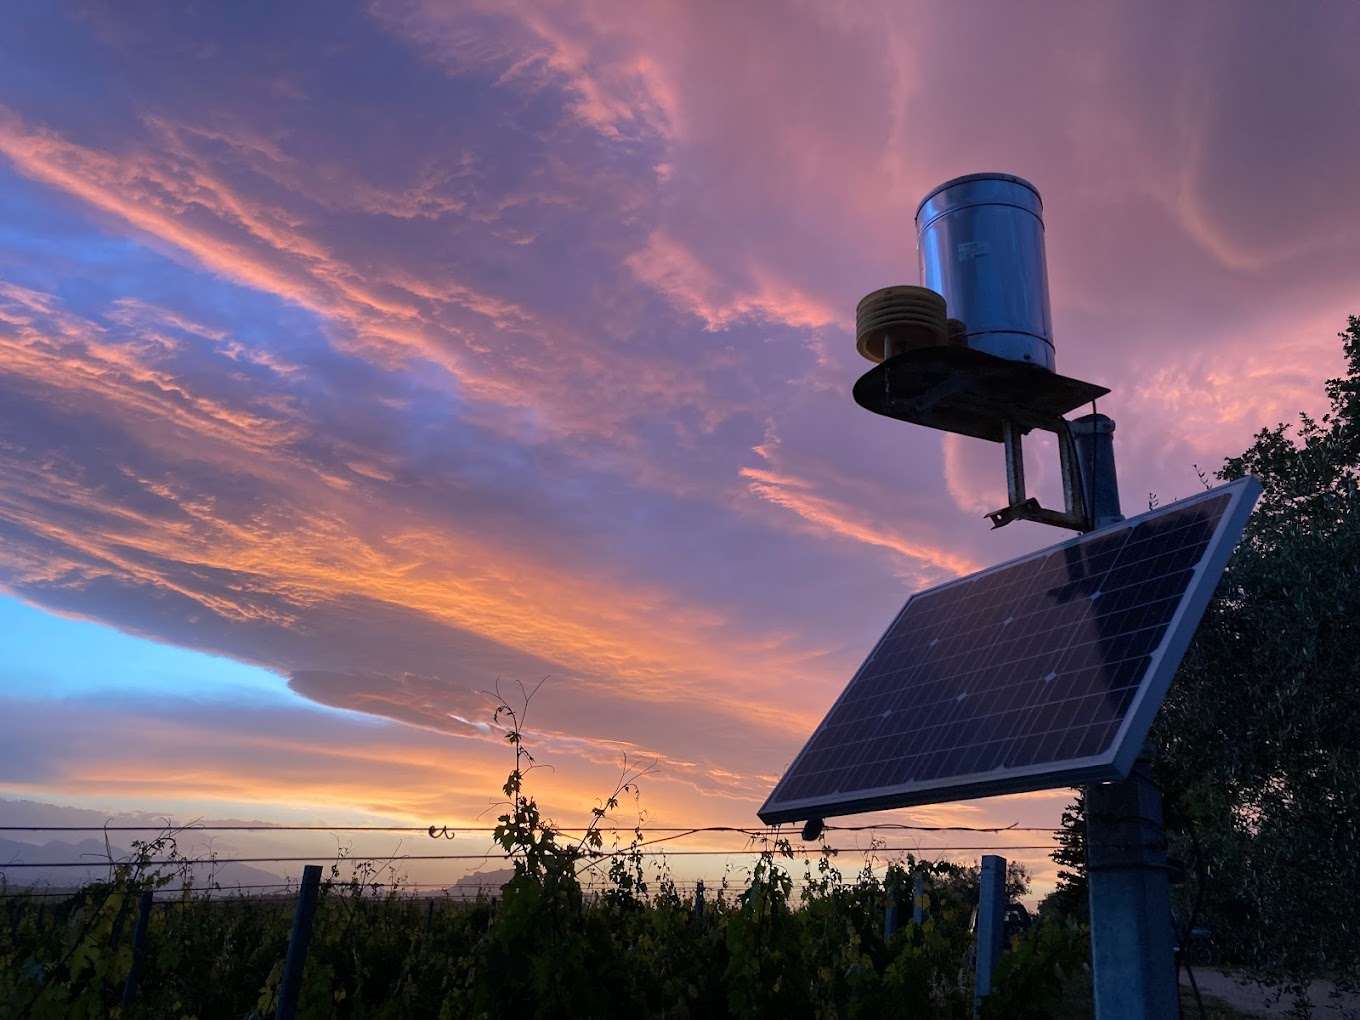
\includegraphics [width=.55\columnwidth, angle=0]
            {stazioneiot}
	\caption{La stazione IoT presente nel campo dell'azienda vitivinicola Strappelli}
	\label{3fig:foto_stazione}
\end{figure}

L'azienda Trace Technologies ha posizionato la stazione IoT nelle vicinanze della vite monitorando i seguenti valori atmosferici e valori utili con lo scopo di stabilire lo stato di salute del vigneto:

\begin{itemize}
    \item temperatura ed umidità atmosferica;
    \item millimetri di pioggia (giornalieri, del giorno precedente, istantanei e totali) misurati tramite un pluviometro posizionato nella parte superiore della stazione (è visibile un contenitore cilindrico nella Figura \ref{3fig:foto_stazione});
    \item temperatura ed umidità della foglia (misurate tramite un sensore mostrato in Figura \ref{3fig:leafSensor});
    \item temperatura ed umidità del terreno (misurate tramite un sensore inserito all'interno del terreno). 
\end{itemize}

\begin{figure}[h]
	\centering
	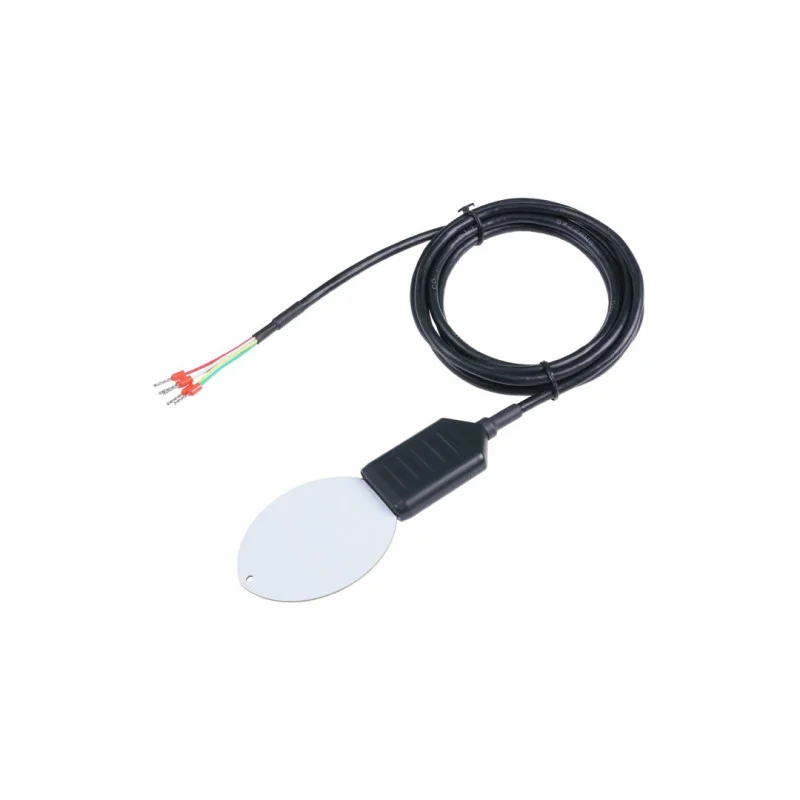
\includegraphics [width=.55\columnwidth, angle=0]
            {leafSensor}
	\caption{Sensore di temperatura ed umidità della foglia}
	\label{3fig:leafSensor}
\end{figure}

Per rendere il progetto sostenibile dal punto di vista ambientale, la stazione IoT è alimentata da un pannello fotovoltaico che durante il giorno fornisce l'energia necessaria alla stazione mentre l'energia che non viene impiegata durante le ore diurne è immagazzinata all'interno di una batteria che alimenta il sistema durante le ore notturne.

La stazione possiede, inoltre, un modulo 3G per la connessione ad Internet tramite una scheda SIM posta al suo interno.

I dati raccolti dalla stazione vengono memorizzati localmente all'interno di una scheda SD per poi essere caricati su una piattaforma cloud che permette l'accesso dei dati da remoto tramite un'apposita API.

\section{Funzionamento dell'applicazione}

Al momento dell'avvio dell'applicazione viene visualizzato un menu che contiene tre pulsanti. Questi ultimi consentono all'utente di selezionare quale delle tre sezioni disponibili (Osserva, Ascolta, Racconta) desidera esplorare dopo che il riconoscimento della bottiglia è stato completato. In Figura \ref{3fig:menuPrincipale} è presente uno screenshot del menù appena descritto.

\begin{figure}[h]
	\centering
	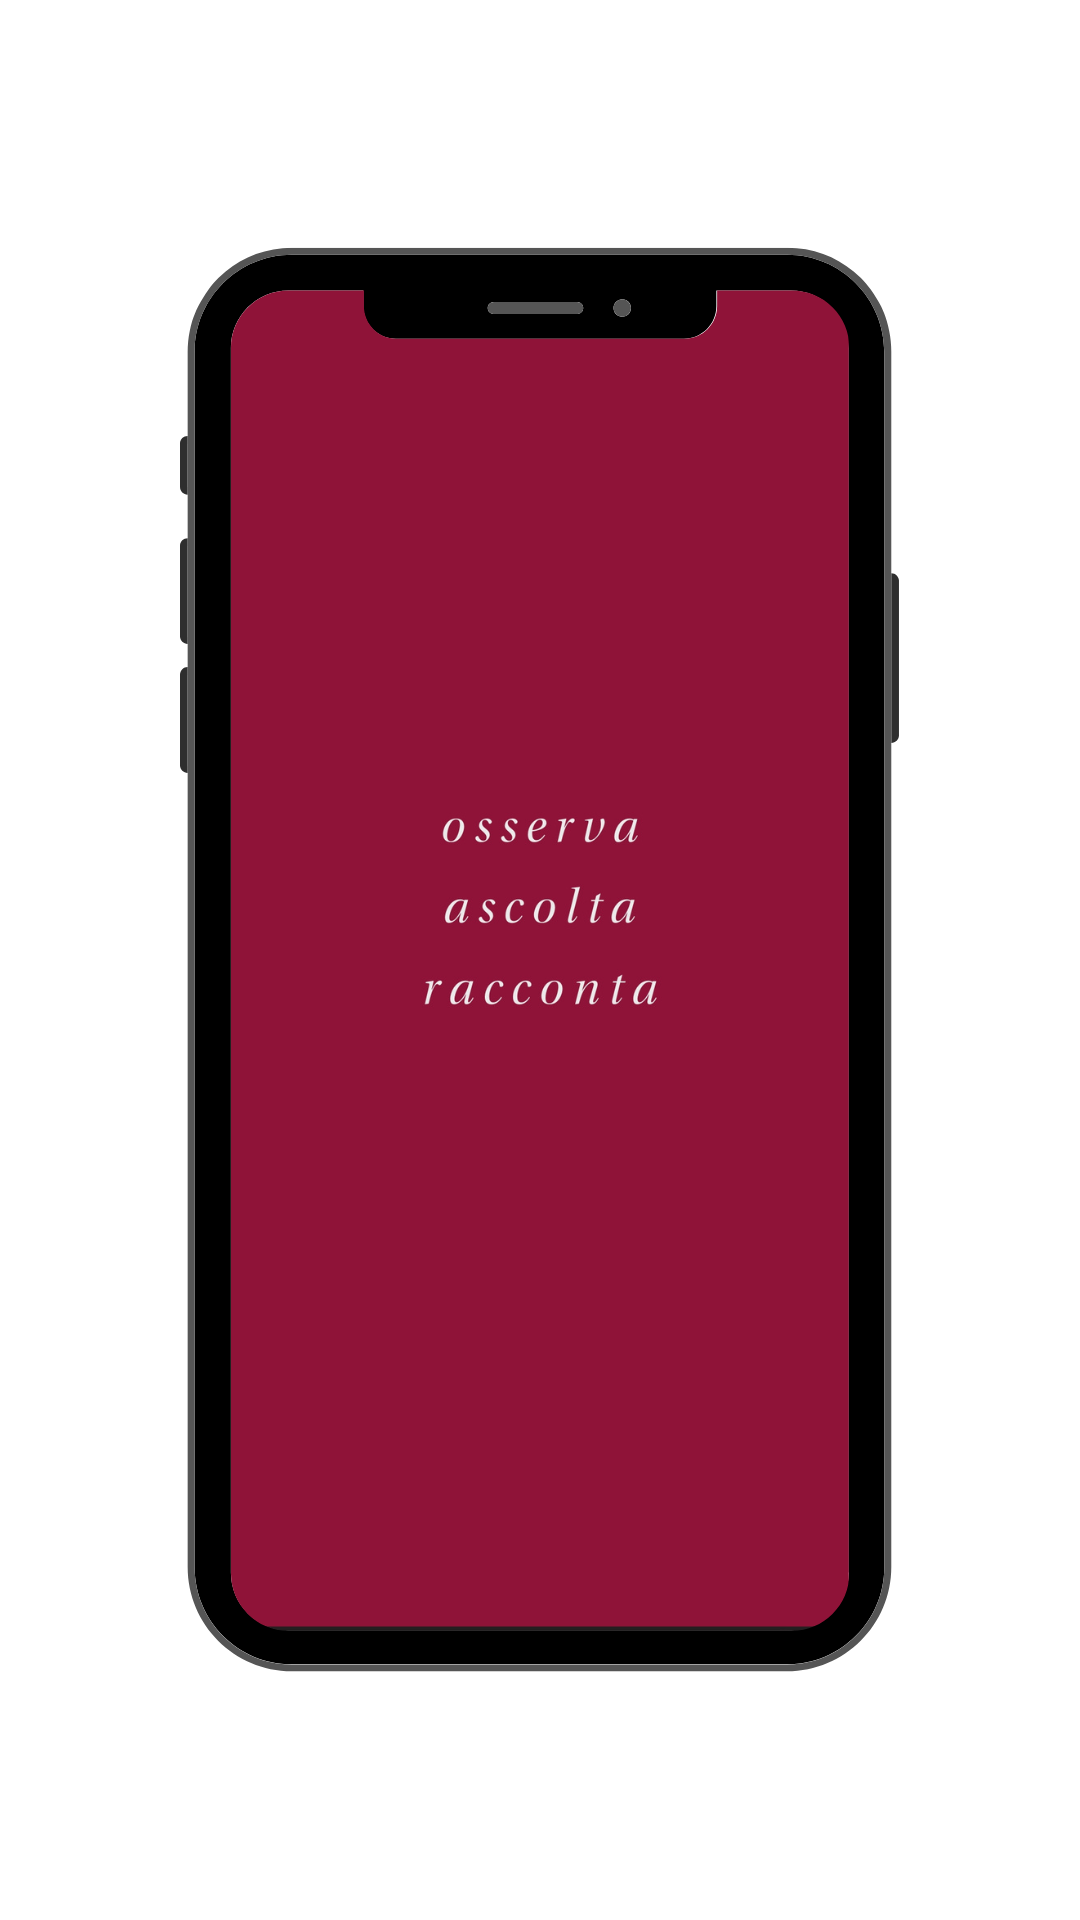
\includegraphics [width=.40\columnwidth, angle=0]
            {menuPrincipale}
	\caption{Menu principale dell'applicazione}
	\label{3fig:menuPrincipale}
\end{figure}

Dopo aver scelto la sezione di interesse, viene mostrata all'utente una schermata composta da un pulsante che permette di accedere alla scena successiva incentrata nell'attivazione della camera AR per il riconoscimento automatico del prodotto vitivinicolo. In Figura \ref{3fig:toccaPerContinuare}, è mostrato il pulsante che attende il tocco dell'utente prima di iniziare il riconoscimento del prodotto.

\begin{figure}[h]
	\centering
	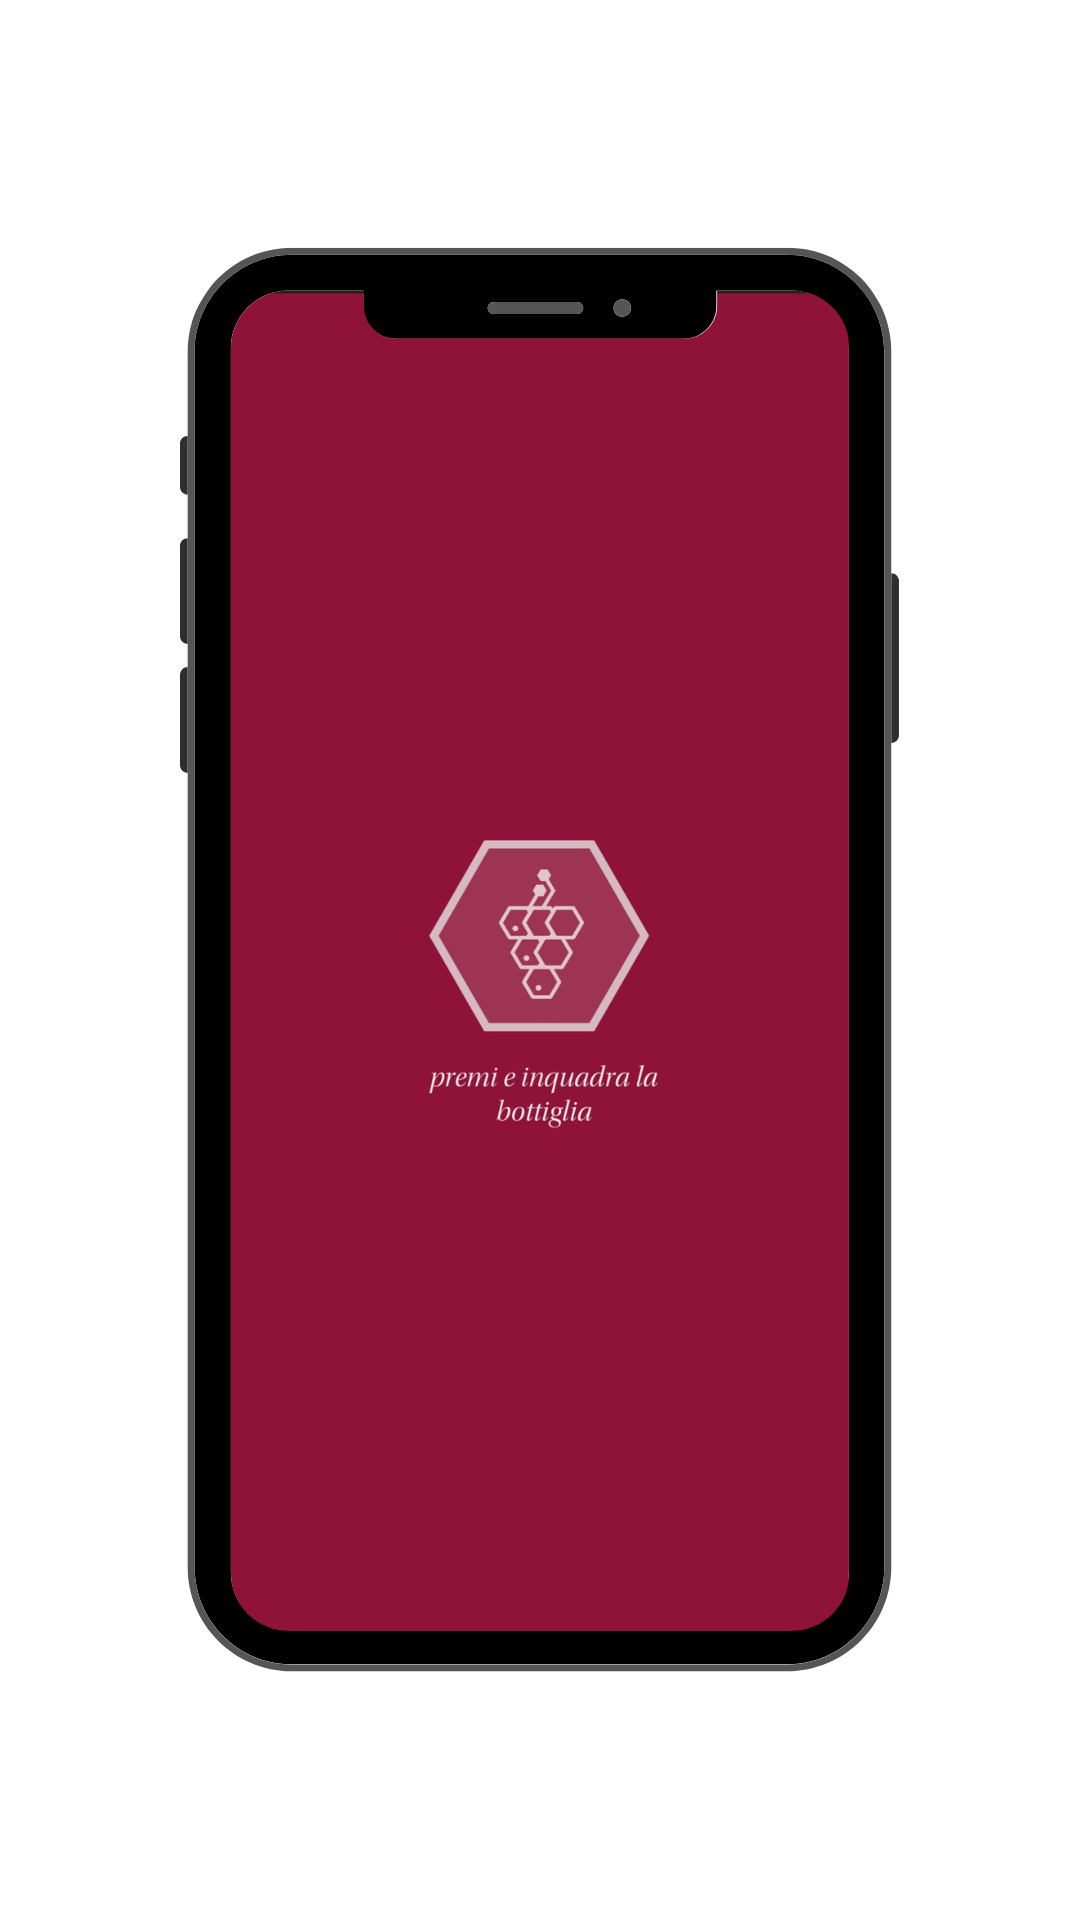
\includegraphics [width=.40\columnwidth, angle=0]
            {toccaPerContinuare}
	\caption{Pulsante che chiede all'utente di iniziare il riconoscimento del prodotto vitivinicolo}
	\label{3fig:toccaPerContinuare}
\end{figure}

Dopo aver premuto uno dei pulsanti, l'applicazione attiva la fotocamera in modalità AR e avvia la ricerca della bottiglia di vino nell'ambiente inquadrato. L'obiettivo è individuare la bottiglia e identificare l'azienda produttrice del vino. Successivamente, l'applicazione mostra le informazioni disponibili sull'azienda, fornite da Trace Technologies. In Figura \ref{3fig:ScenaRiconoscimento} è mostrato uno screenshot della scena Unity.

\begin{figure}[h]
	\centering
	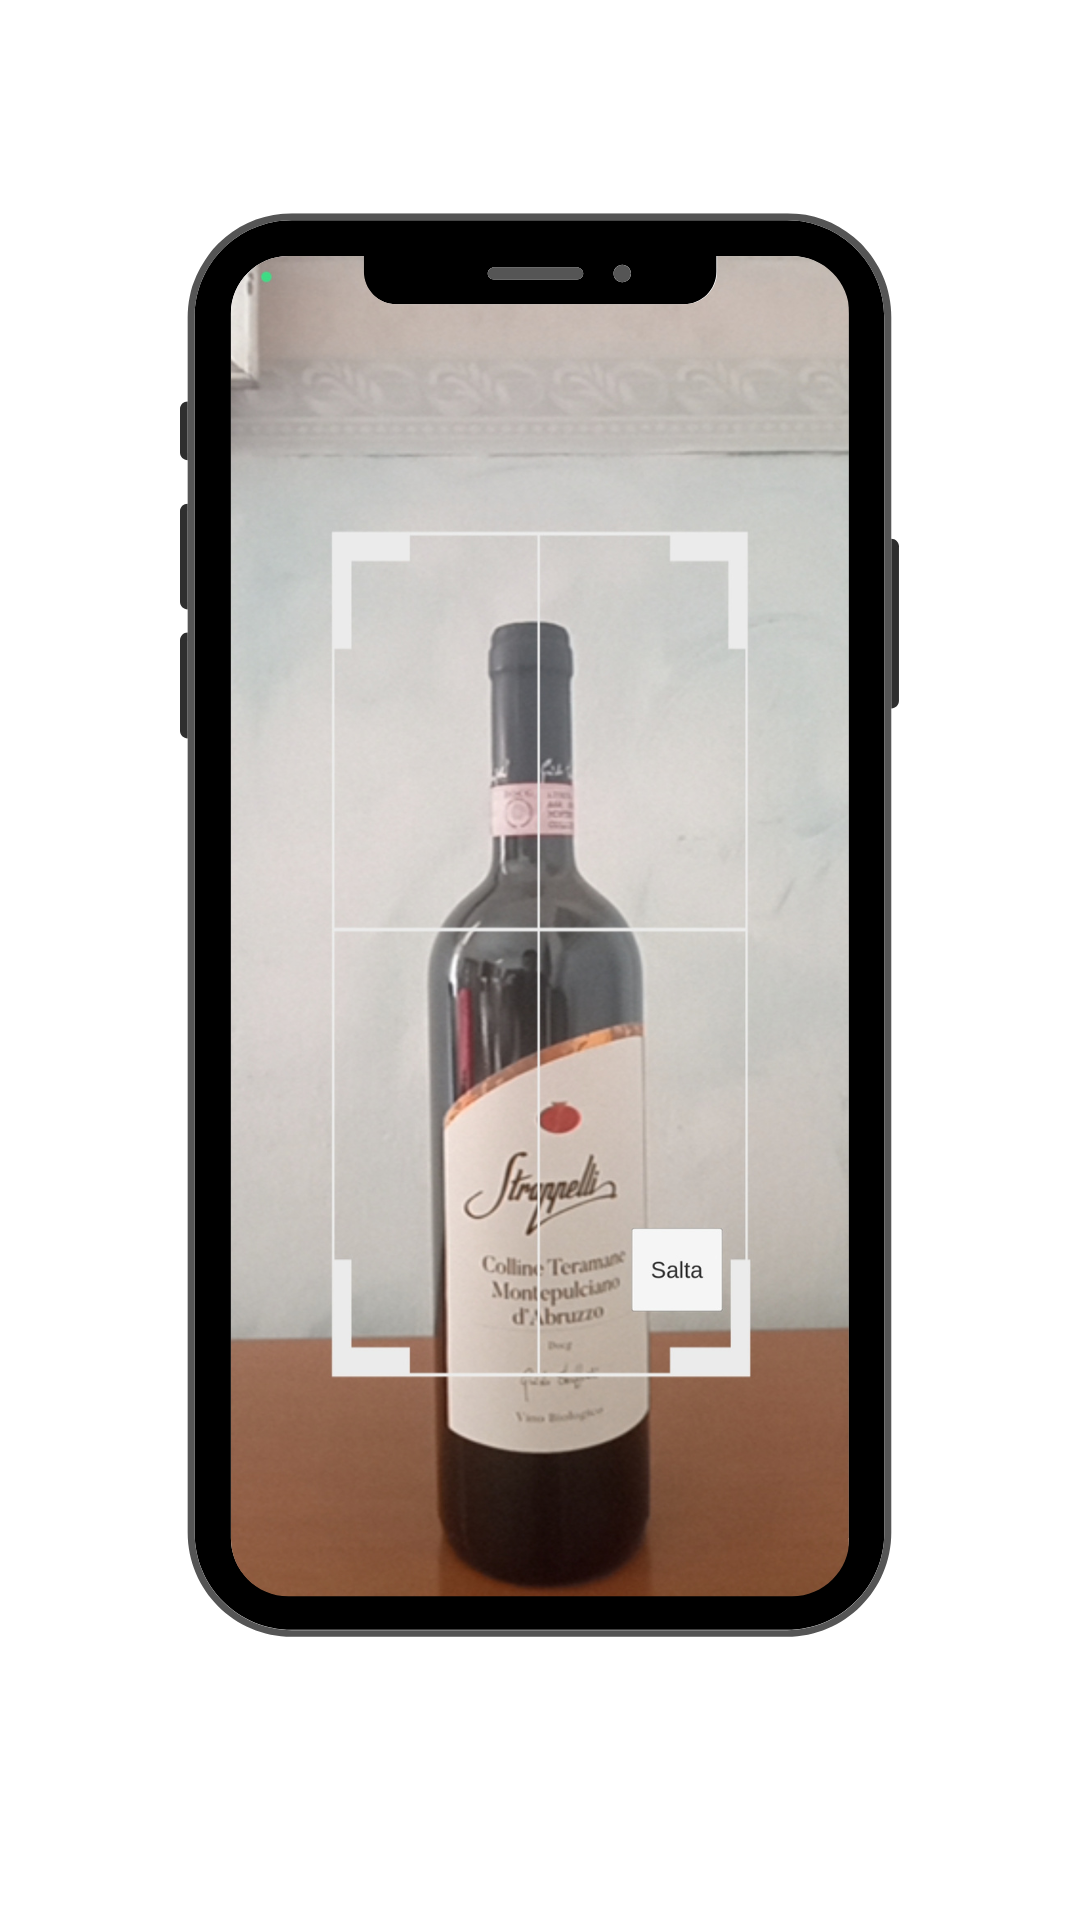
\includegraphics [width=.40\columnwidth, angle=0]
            {ScenaRiconoscimento}
	\caption{Scena AR dedicata al riconoscimento del prodotto vitivinicolo}
	\label{3fig:ScenaRiconoscimento}
\end{figure}

Per scopi dimostrativi, è stato incluso nell'applicazione un pulsante denominato "salta", il quale consente di procedere alla scena successiva anche se la bottiglia di vino non è stata riconosciuta. In situazioni in cui l'utente non possiede effettivamente la bottiglia di vino, verrà impostata una variabile che registra il tag della bottiglia riconosciuta con il valore "Strappelli".

Una volta completato il processo di riconoscimento della bottiglia, l'applicazione Unity passa ad una nuova scena. In quest'ultima, la fotocamera rimane attiva ma l'algoritmo di riconoscimento degli oggetti viene disattivato per risparmiare risorse. Successivamente, viene mostrata una finestra a comparsa dall'alto che chiede all'utente di selezionare l'annata della bottiglia che possiede. Questa scelta implementativa è stata necessaria poiché Vuforia Engine non è sempre in grado di determinare con precisione l'annata della bottiglia dall'etichetta, poiché quest'ultima potrebbe non essere sempre chiaramente visibile.

In Figura \ref{3fig:FinestraScorrevole} è mostrata la finestra scorrevole appena descritta.

Selezionata l'annata, l'applicazione Unity carica l'ultima scena che contiene tutte le sezioni menzionate in precedenza (Osserva, Ascolta e Racconta) mostrate, rispettivamente, nelle Figure \ref{3fig:ScenaOsserva}, \ref{3fig:ScenaAscolta} e \ref{3fig:ScenaRacconta}.

\begin{figure}[h]
	\centering
	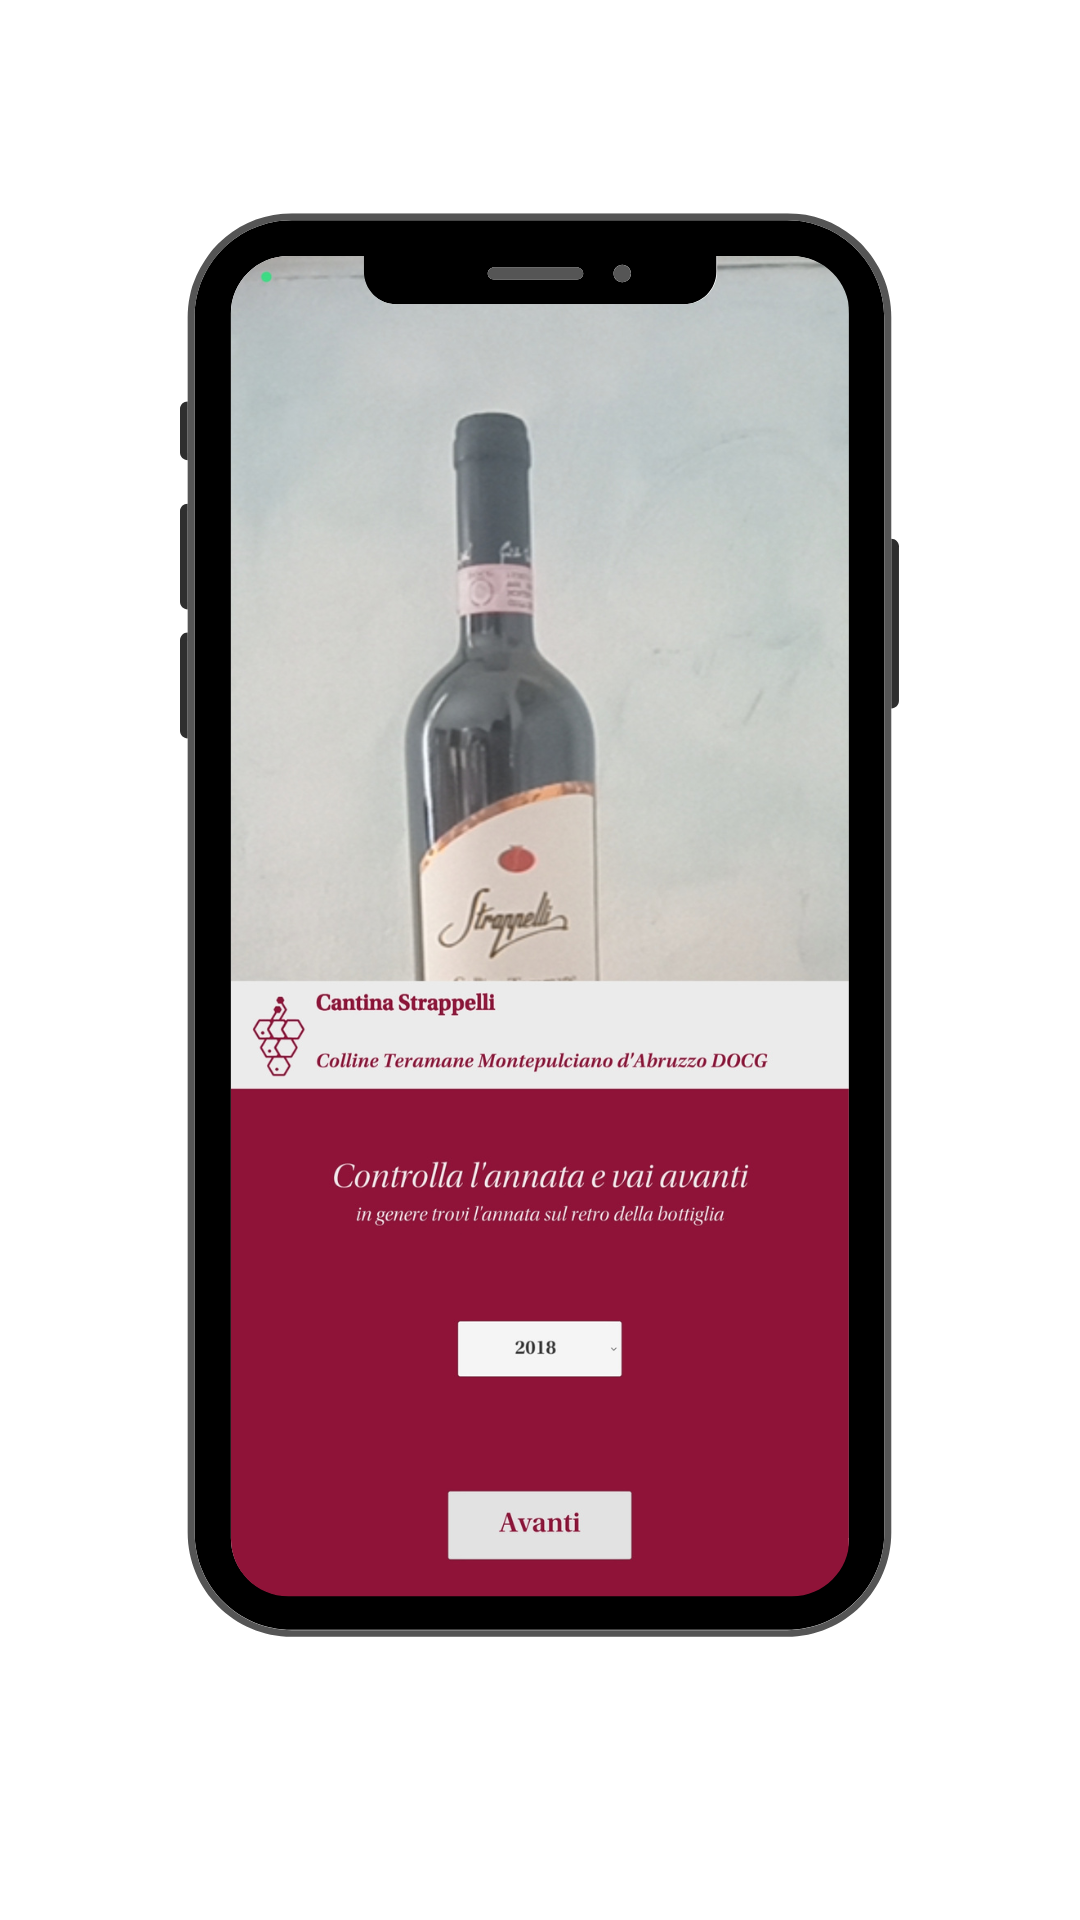
\includegraphics [width=.40\columnwidth, angle=0]
            {FinestraScorrevole}
	\caption{Finestra per la selezione dell'annata del prodotto vitivinicolo}
	\label{3fig:FinestraScorrevole}
\end{figure}

\begin{figure}[h]
	\centering
	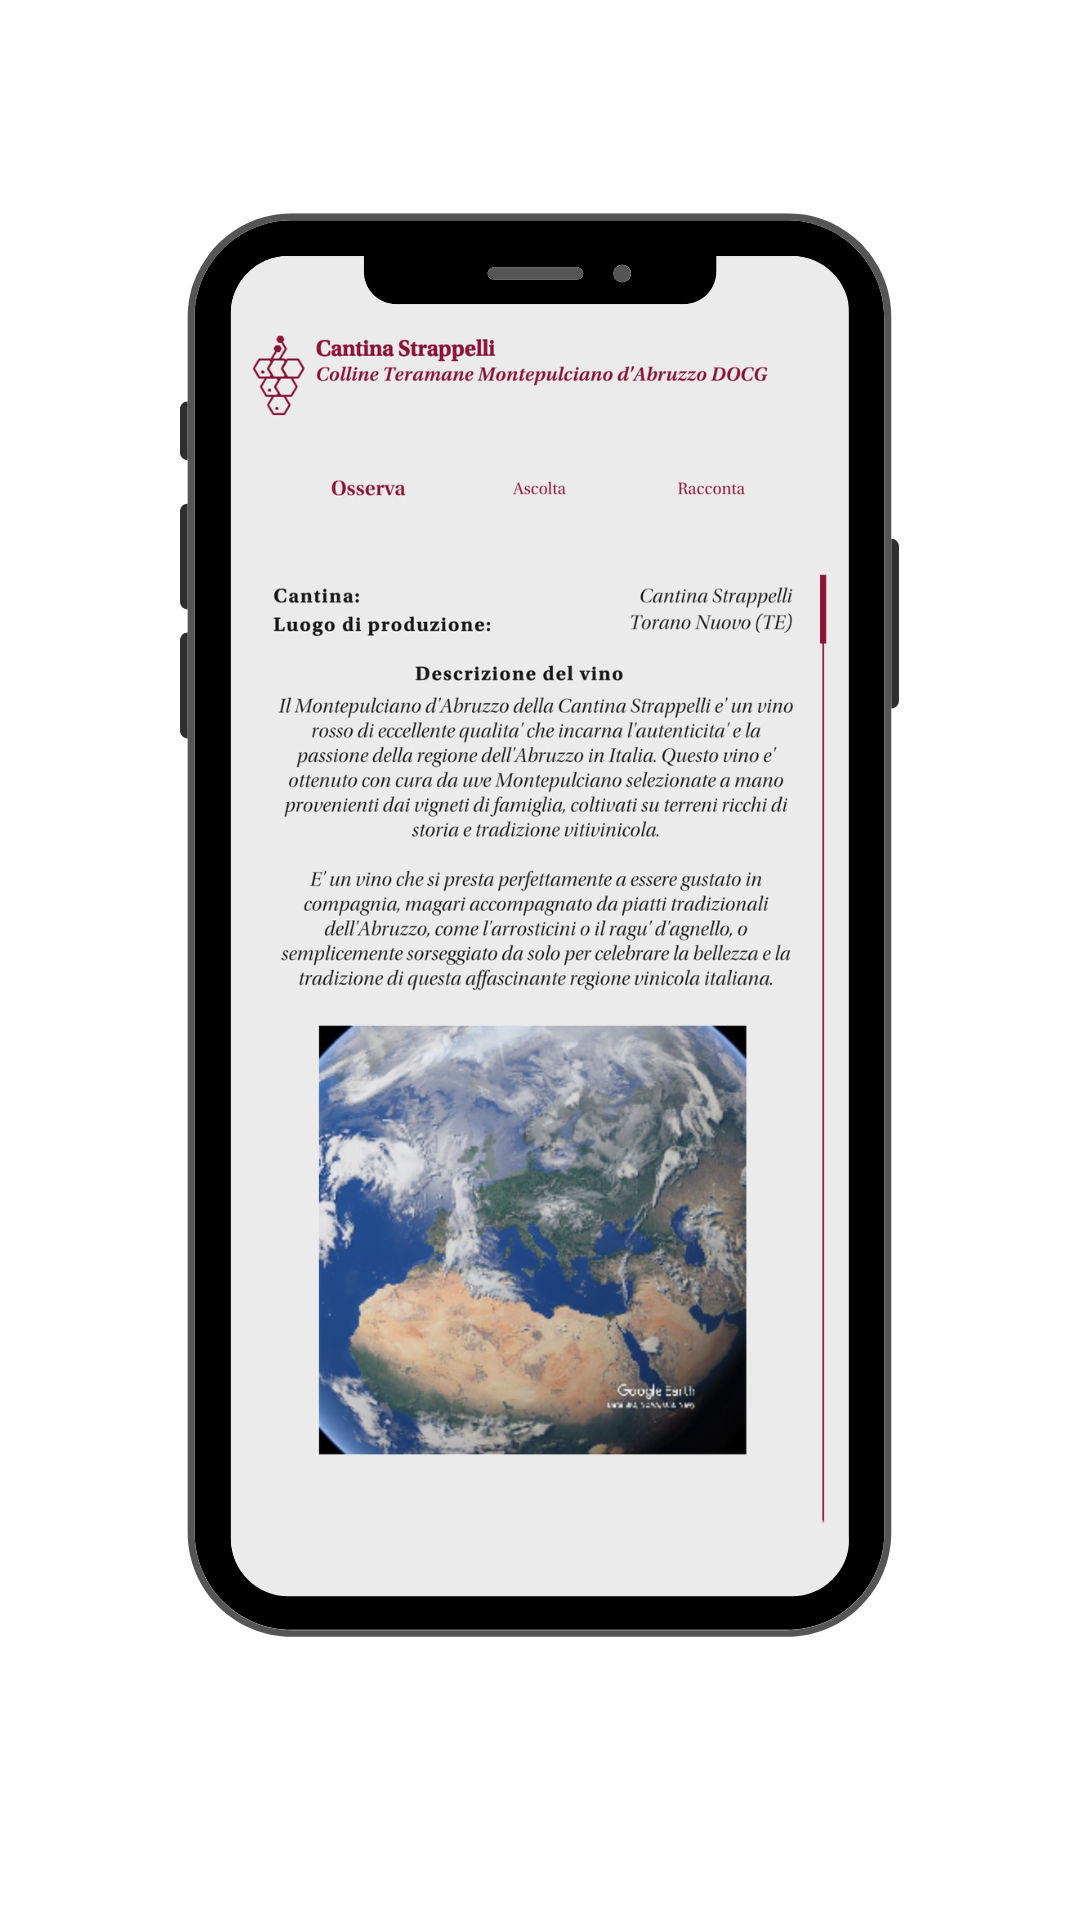
\includegraphics [width=.40\columnwidth, angle=0]
            {ScenaOsserva}
	\caption{Screenshot della sezione Osserva}
	\label{3fig:ScenaOsserva}
\end{figure}

\begin{figure}[h]
	\centering
	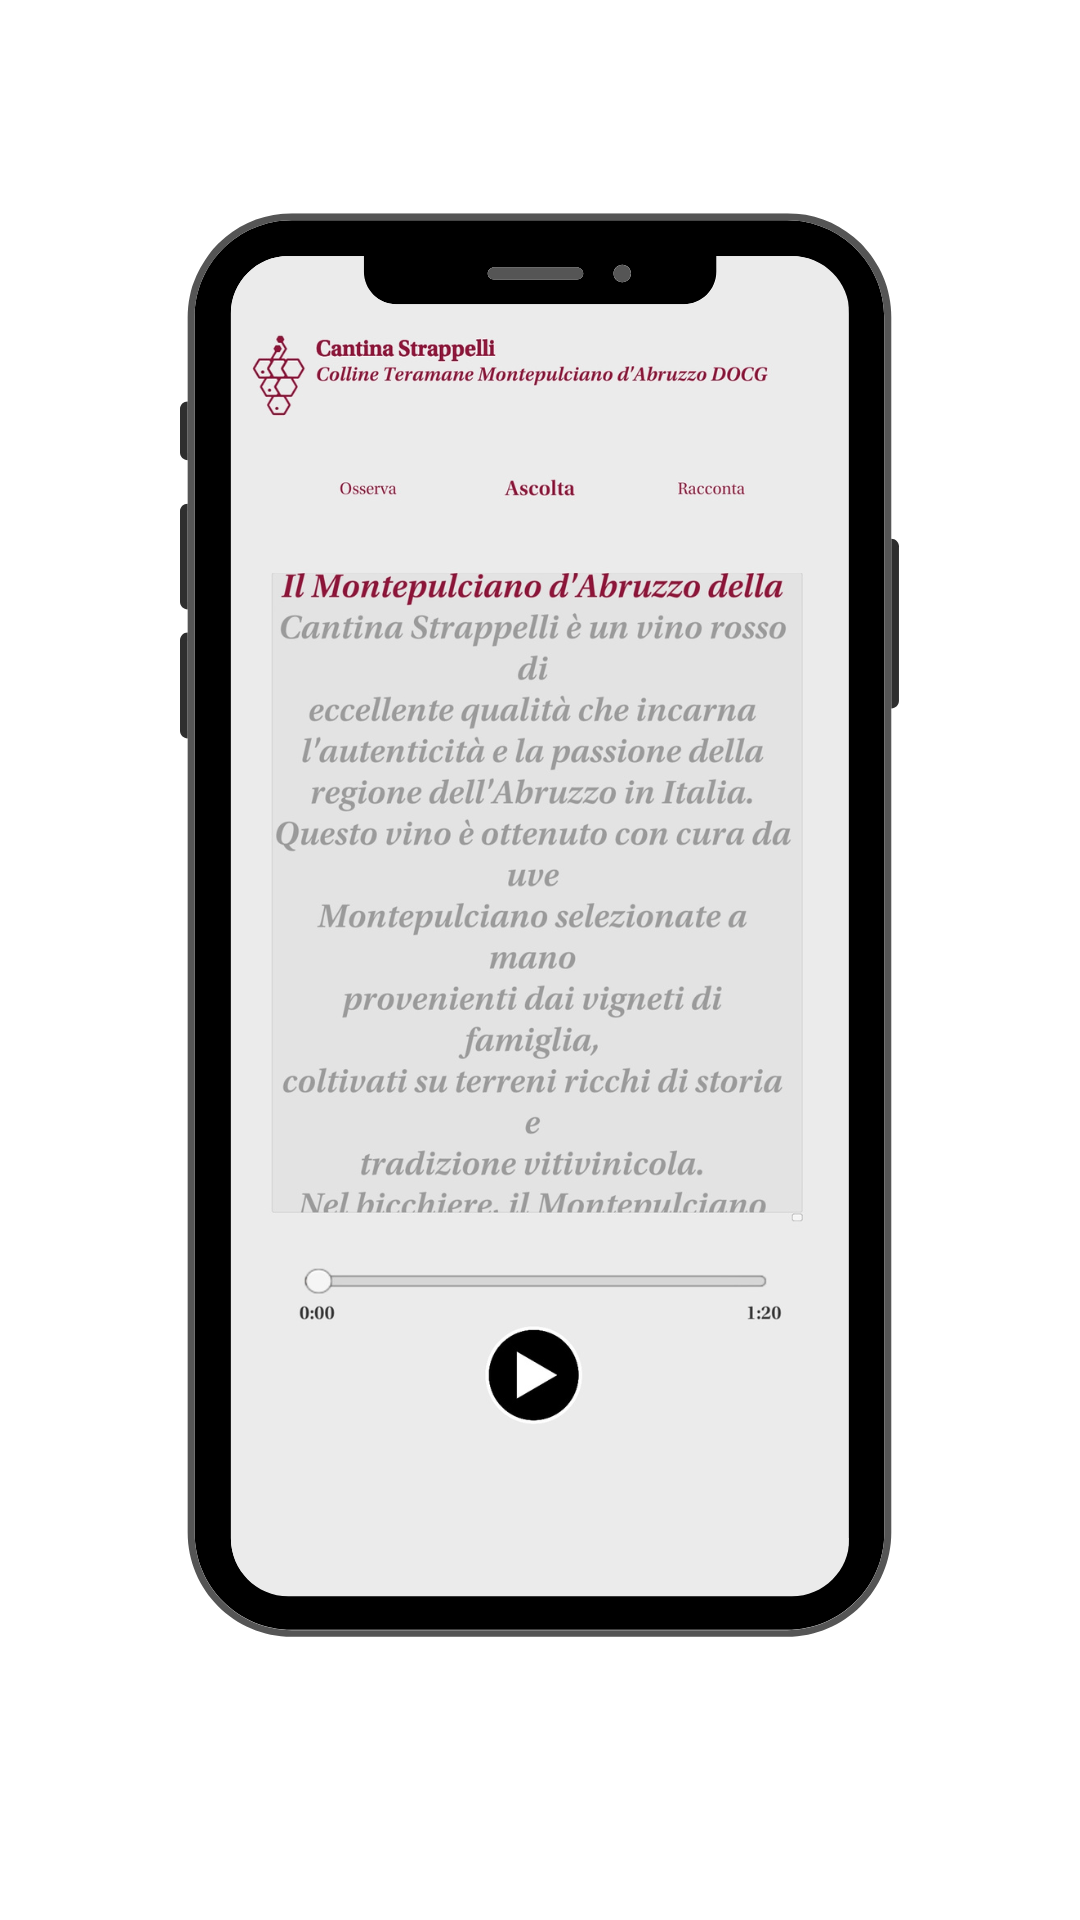
\includegraphics [width=.40\columnwidth, angle=0]
            {ScenaAscolta}
	\caption{Screenshot della sezione Ascolta}
	\label{3fig:ScenaAscolta}
\end{figure}

\begin{figure}[h]
	\centering
	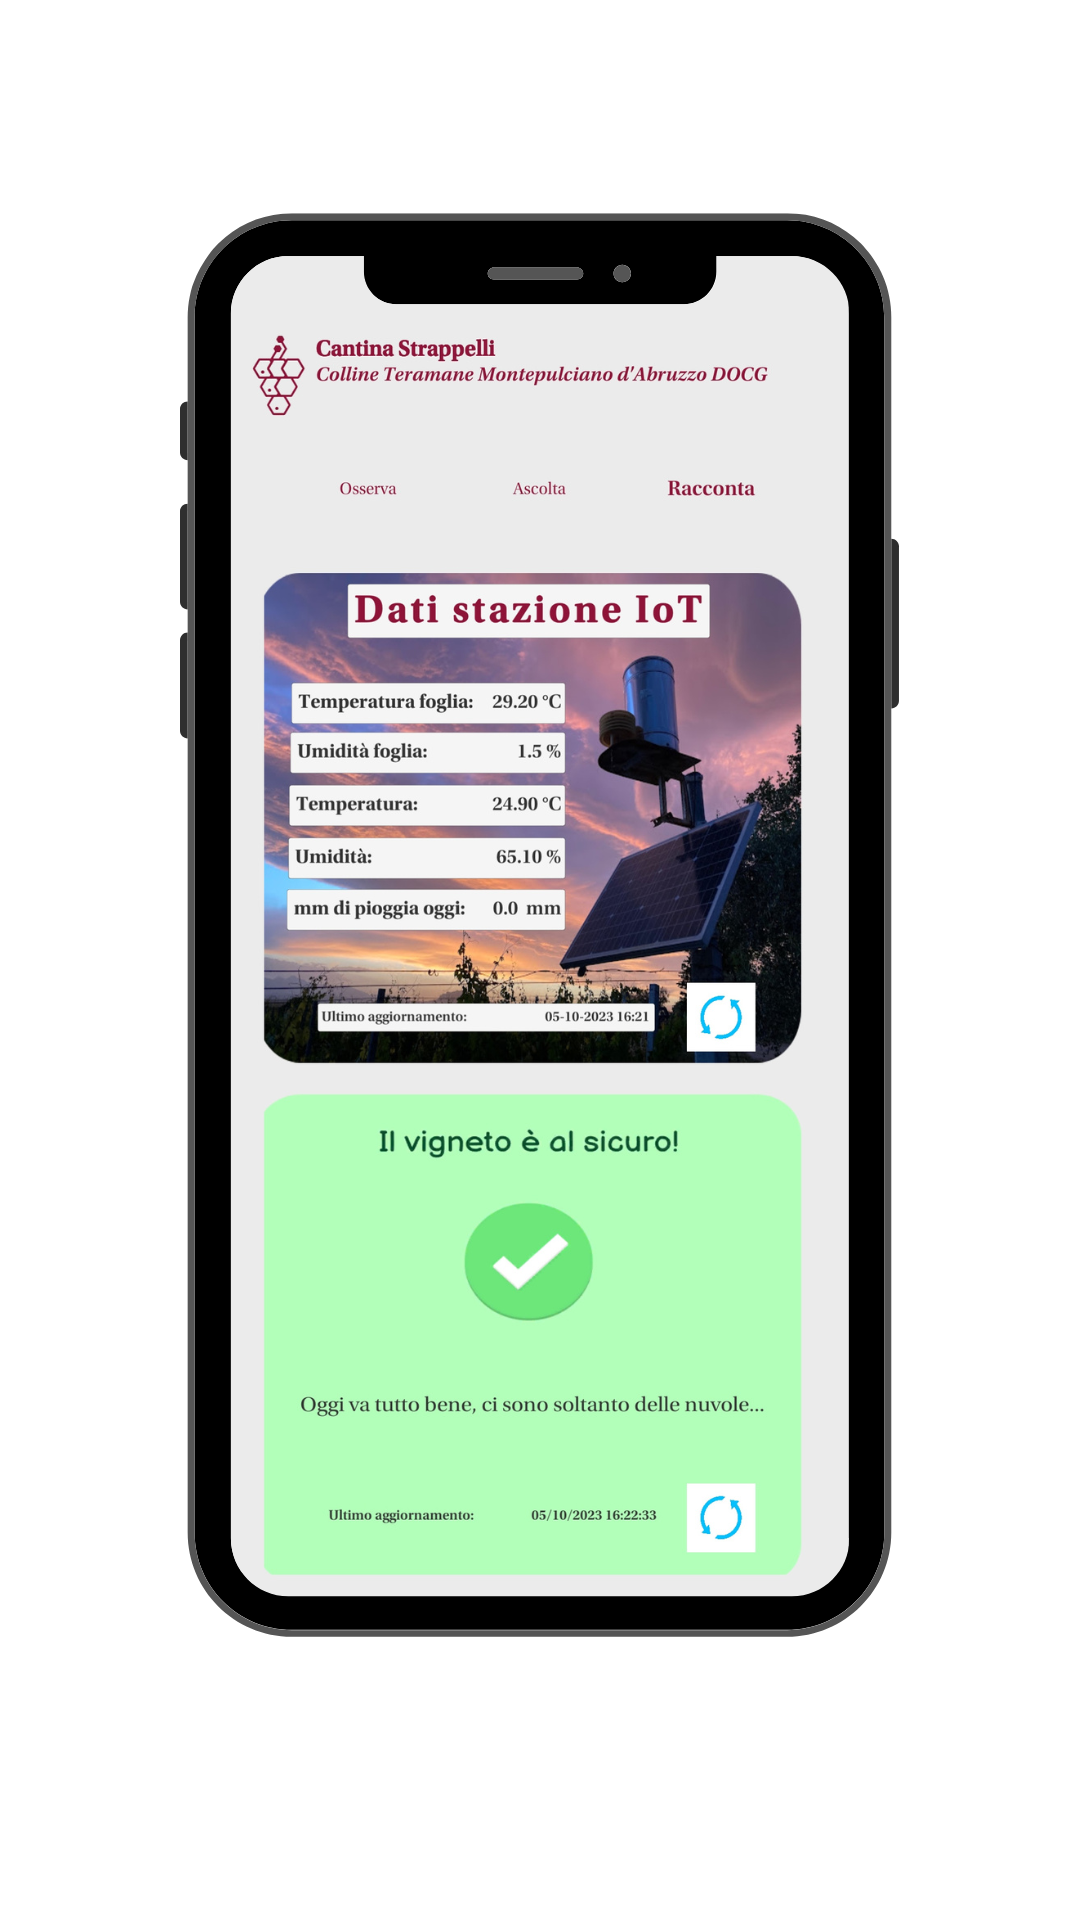
\includegraphics [width=.40\columnwidth, angle=0]
            {ScenaRacconta}
	\caption{Screenshot della sezione Racconta}
	\label{3fig:ScenaRacconta}
\end{figure}